\pdfoutput=1
\documentclass[10pt]{beamer}

%STANDARD PREAMBLE
%https://tex.stackexchange.com/questions/68821/is-it-possible-to-create-a-latex-preamble-header
\usepackage{../../rsrc/beamer_preamble}

% EMBED ANIMATIONS
% Reference: https://tex.stackexchange.com/questions/240243/getting-gif-and-or-moving-images-into-a-latex-presentation
%\usepackage{xmpmulti}
\usepackage{animate}

%%% SPECIFIC TO THIS DOC
\newcommand{\obs}{x^{(i)} }
\newcommand{\alatent}{z^{(i)} }
\newcommand{\I}{\mathbb{I}}





\title{Normalizing Flows}

\begin{document}

\maketitle

\begin{frame}{Table of contents}
  \setbeamertemplate{section in toc}[sections numbered]
  \tableofcontents[hideallsubsections]
\end{frame}

\section{Overview}
 
\begin{frame}{Main Idea}
  \animategraphics[loop,controls,width=\linewidth]{10}{movie_frames/two_moons-}{1}{30}

\scriptsize
\textit{Normalizing flows} provide a general mechanism for defining expressive probability distributions, only requiring the specification of a (usually simple) base distribution and a series of
bijective transformations.
\vfill
\tiny \hfill Animation Credit: Mike Slawinski, Ph.D., Cylance, Inc.
\end{frame}
    
\begin{frame}{}

\begin{figure}[H]
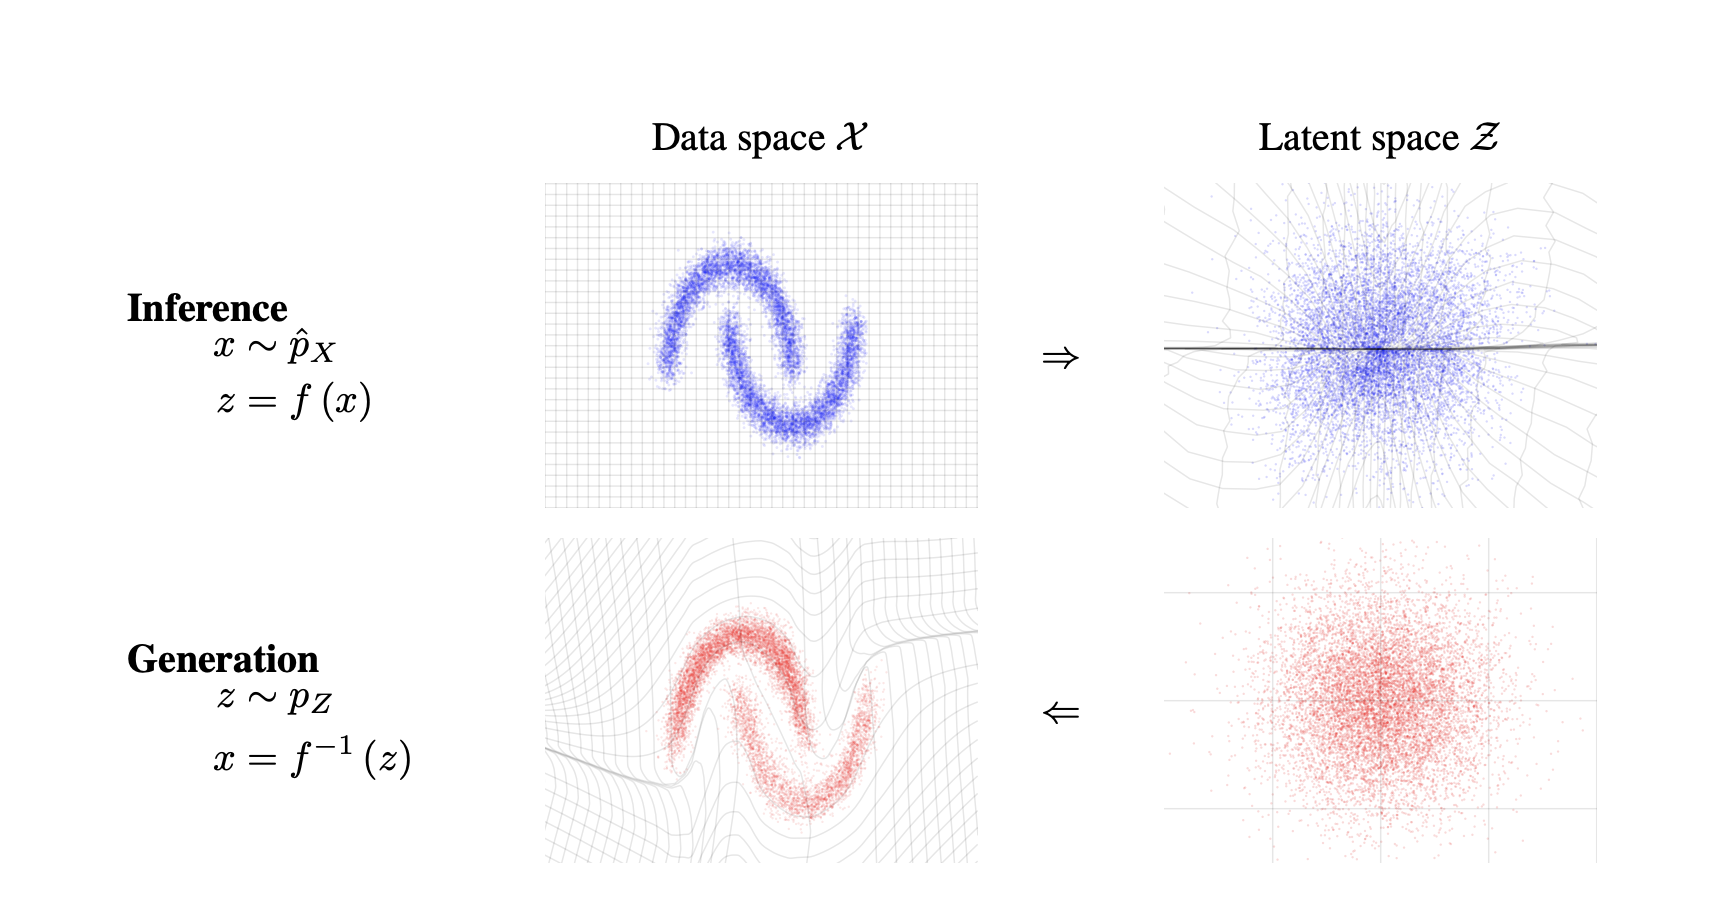
\includegraphics[width=\textwidth]{images/nf_idea}
\end{figure} 
We learn an invertible mapping $f$ between a data distribution $\widehat{p}_X$ and a latent distribution $p_Z$ (typically a Gaussian).  The technique allows one to perform anomaly detection and sample generation even for complex and high-dimensional distributions.
\vfill
\tiny \hfill Image Credit: Dinh et al. (2017), ICLR. 
 \end{frame}
 
 
\begin{frame}{Application: Sample Generation}
\begin{figure}[H]
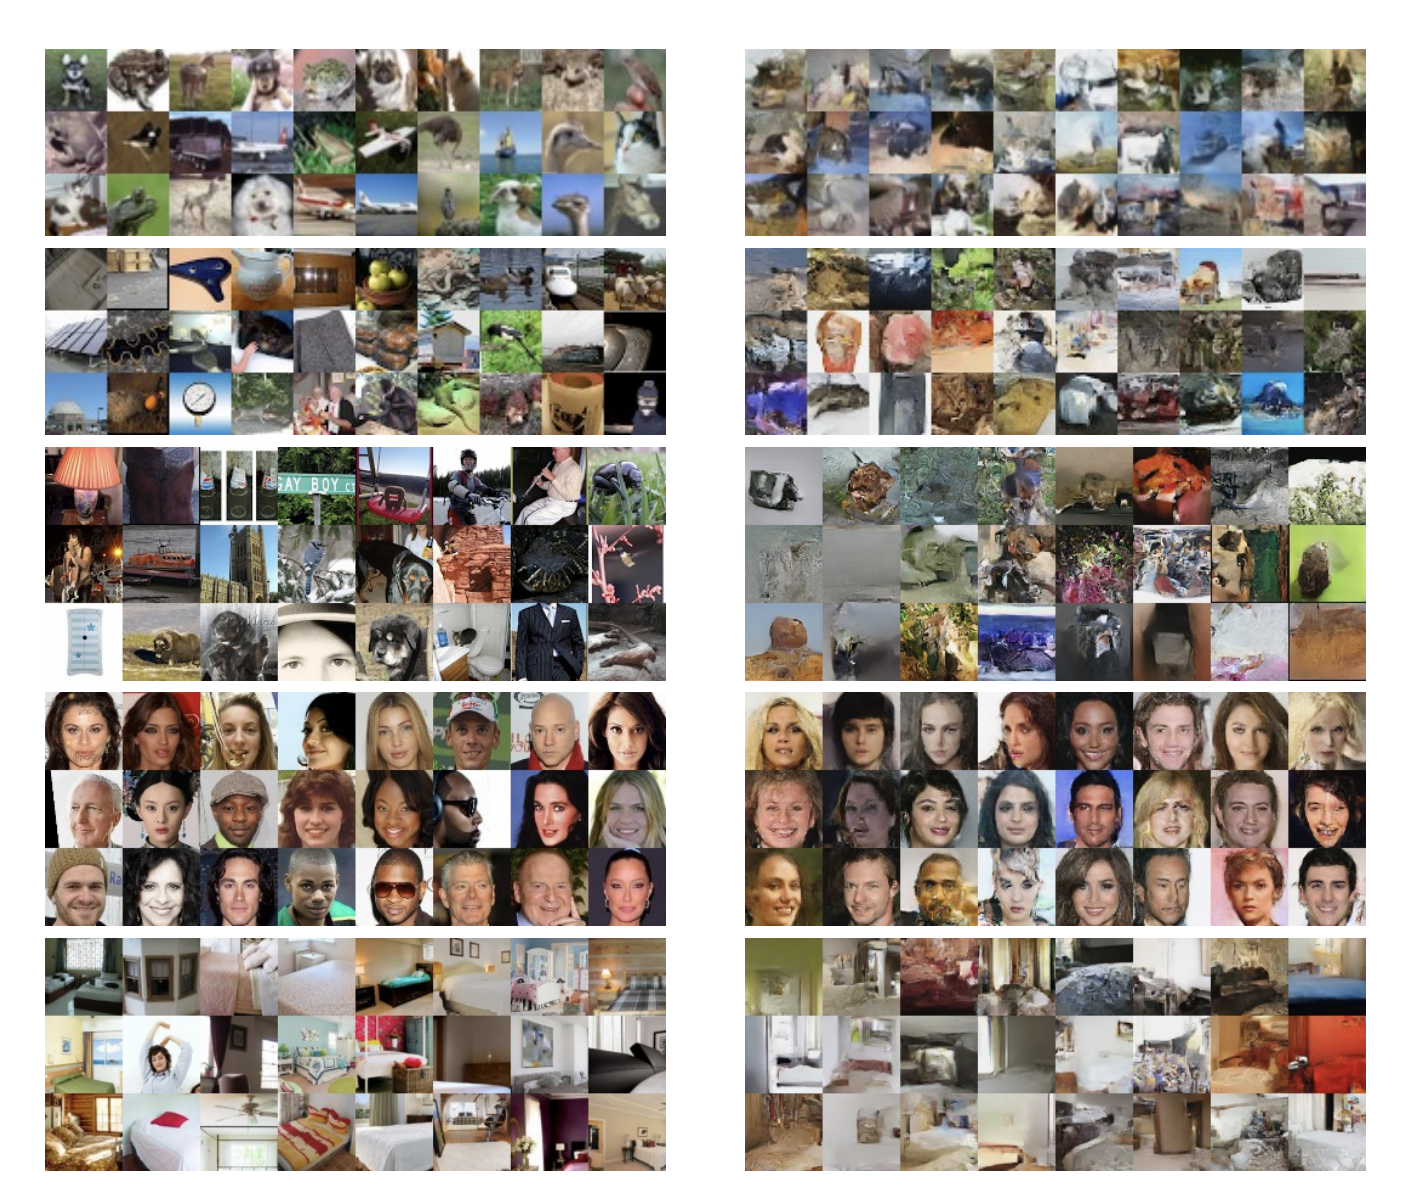
\includegraphics[width=.8\textwidth]{images/nf_image_samples}
\end{figure} 
\scriptsize On the left column, examples from a dataset. On the right column, samples from a normalizing flow model trained on the dataset.  \tiny The datasets shown in this figure are in order: CIFAR-10, Imagenet
(32 × 32), Imagenet (64 × 64), CelebA, LSUN (bedroom).
\vfill
\tiny \hfill Image Credit: Dinh et al. (2017), ICLR. 
 \end{frame}

\begin{frame}{Application: Anomaly Detection in Cybersecurity}
\pause
\scriptsize
\textit{String stuffing} attacks can fool ML-based Antivirus into thinking malware is good.   %\tiny Similar attacks can be used to get past spam-filters in e-mail. \scriptsize 

\begin{figure}[H]
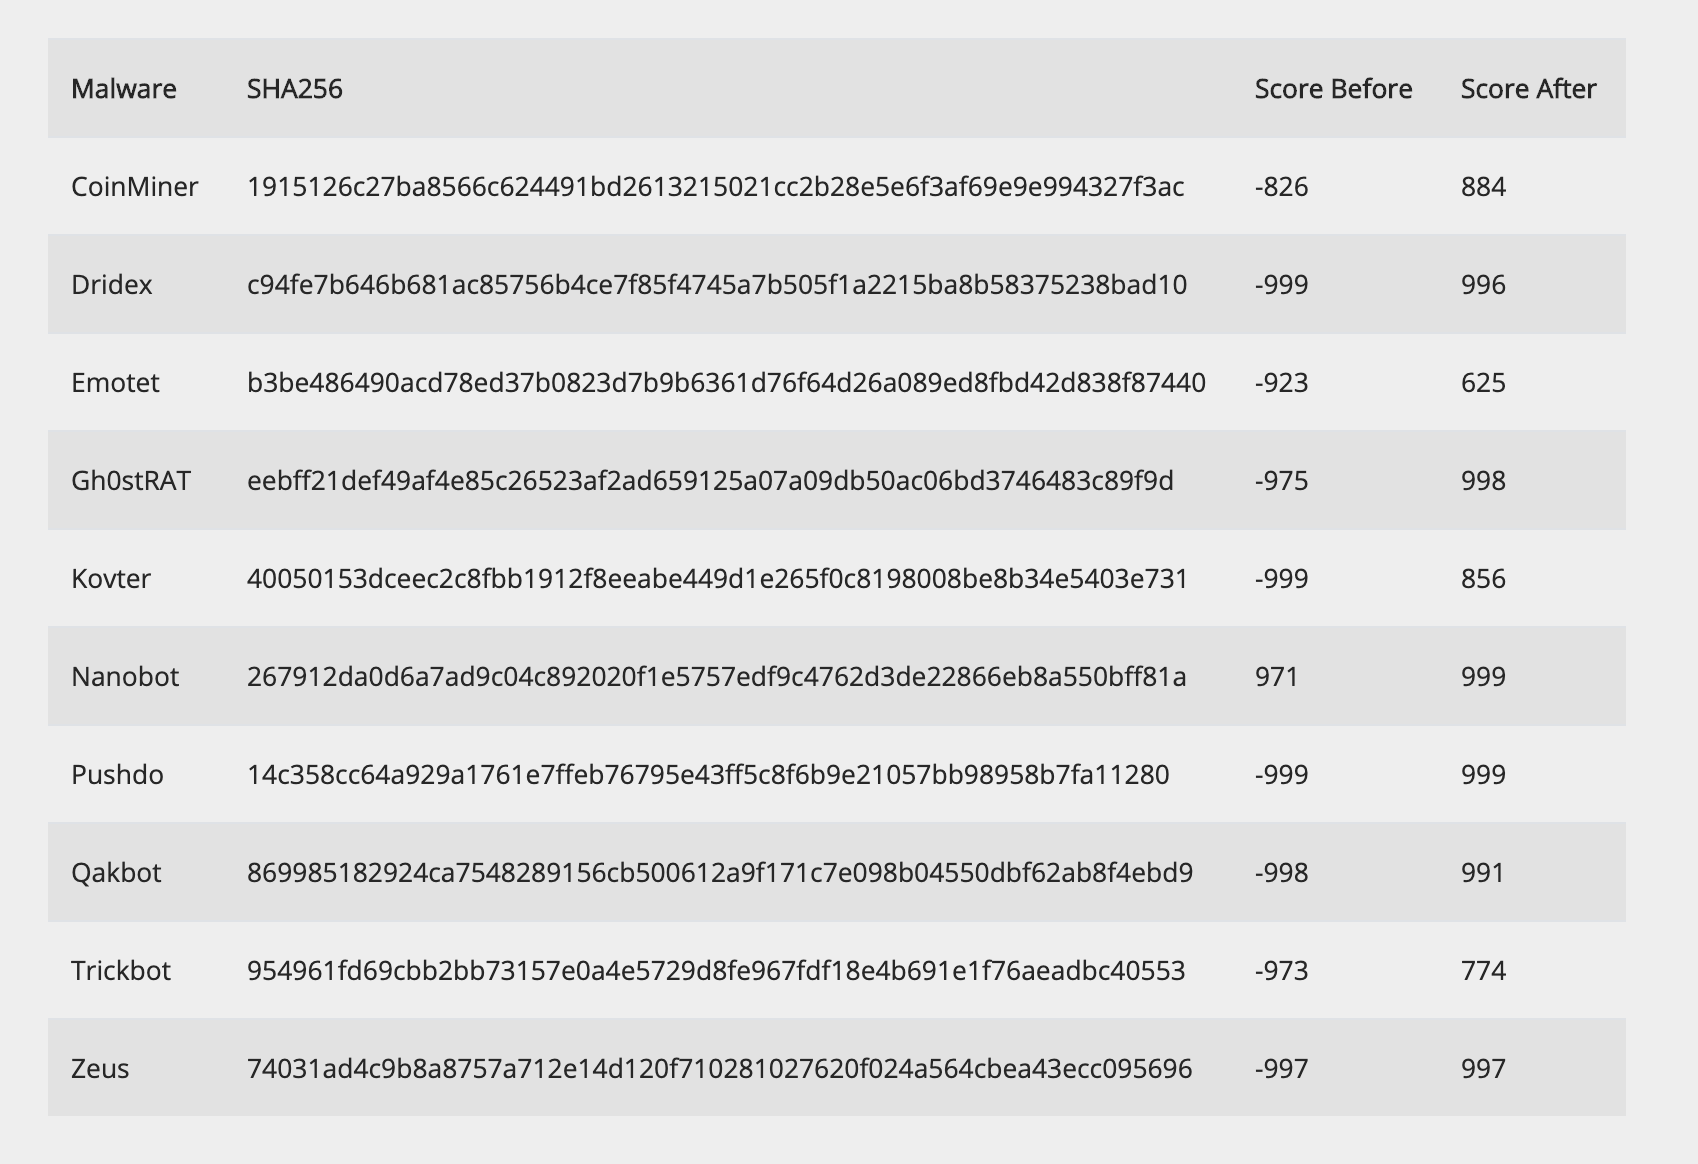
\includegraphics[width=.75\textwidth]{images/string_stuffing}
\end{figure} 

However, these Frankensteinian concoctions look anomalous in feature space.
 
\vfill \vfill \vfill
\tiny \hfill Reference: \url{https://skylightcyber.com/2019/07/18/cylance-i-kill-you/}

\end{frame}



\section{Density estimation and change of variables} 

\begin{frame}
Consider a parametric function mapping continuous random variable $X$ to continuous random variable $Z$

\begin{align*}
f_\theta:  &\, X \to Z \\
			&\, x \mapsto z 
\end{align*}

where $x$ is an observed sample and $z$ is a latent variable.  Suppose $p_Z$ is given.   
\vfill
Under some regularity conditions\footnote{Importantly, $f_\theta$ must be a \textit{diffeomorphism} -- i.e. it must be invertible, and both it and its inverse must be differentiable}, the change of variables theorem gives us

\[ \labeledgreenbox{data \; space}{$p_X(x)$} = \labeledbluebox{transformed \; latent \; space}{$p_Z( f_\theta(x) ) \absdet{\df{\partial f_\theta(x)}{\partial x}}$}  \]  
\end{frame}

\begin{frame}
The \textbf{goal} of density estimation can be posed as follows: learn $\theta$ to model unknown data density $p_X$ in terms of assumed latent variable density $p_Z$.   \\
\pause 
\vfill \vfill \vfill 
The \textbf{problem} is that for high-dimensional data, computing the Jacobian and determinant is in general computationally very expensive.\footnote{E.g., straightforward computation of the determinant via LU decomposition is $\mathcal{O}(d^3)$, where $d$ is the dimensionality of the data.} \\
\pause 
\vfill \vfill \vfill 
There appears to be a \textbf{conflict} between expressivity and efficiency.
\end{frame}



\section{Normalizing Flow} 

\begin{frame}
\begin{definition}{(Normalizing Flow)} \label{flow}
A \textit{(normalizing) flow}, $f=h_\theta^1 \circ ... \circ h_\theta^K$, is a sequence of diffeomorphisms which maps an observed data point, $x$, to a latent state representation, $z$. 
\end{definition}

\pause
If we allow ourselves this abuse of notation\footnote{More generally, we will use the same notation to refer to the function itself as well as its evaluation at a point.}
\begin{align*}
h_\theta^0 &:=x \\
h_\theta^K &:= z \\
\end{align*}

Then, since $\det \prod_i A_i = \prod_i \det A_i$, the likelihood becomes 

\begin{equation} 
\label{cov}
p_X(x) = p_Z( f_\theta(x) ) \ds\prod_{k=1}^K\absdet{\df{\partial h_\theta^k}{\partial h_\theta^{k-1}}}  
\end{equation}
\end{frame}

%A flow-based generative model assumes $p_\theta(z)$ is tractable, e.g. a spherical multivariate Gaussian.  Then, by the change of variables formula, we can use $f$ and its inverse $g := f^{-1}$ to compute the probability density $p_\theta(x)$.   Training the model means learning $\theta$ to maximize the likelihood
%
%\[ p_X(x) = p_Z(z) \absdet{\df{\partial f(x)}{\partial x^T}}  \] 
%
%where we have used the change of variables to express density $p_X$ in terms of density $p_Z$.  


%\begin{definition}{(Coupling layer)} \label{coupling_layer}
%\red{to do}
%\end{definition}

%%%%%%%%%%%%%%%%%%%%%%%%%%%%%%%%%%%%%%%%%%%
%%%%%%%%%%%%%%%%%%%%%%%%%%%%%%%%%%%%%%%%%%%
\section{Real NVP}

\begin{frame}{Idea}
 \textbf{Real non-volume preserving flows} (RNVP; Dinh et al., 2016) is a normalizing flow where  each bijection in the sequence of bijections works in the following way. 
 
 \begin{itemize}
 \item The d features of a random variable are partitioned into two groups.   \pause 
	 \begin{itemize}
	 \item The first  group is transformed by the identity transformation. \pause
	 \item The second group is transformed by a more complex operation whereby its values are scaled and translated (hence, an \textit{affine transformation}) by factors created by applying neural networks to the features in the first group (hence, a \textit{coupling transformation}).  \pause
	 \end{itemize}

 \end{itemize}
\vfill
Each such bijection is called an "affine coupling transformation" or "affine coupling layer" (ACL).
\end{frame}


\begin{frame}
\begin{definition}{(Real NVP)} \label{rnvp}
A \textit{real NVP} is a normalizing flow (Def. \ref{flow}) where $f=h_\theta^1 \circ ... \circ h_\theta^K$ is structured such that:

\[h^{k+1} = b^k \odot h^k + (1-b^k) \odot \bigg( h^k \odot \exp \big( s^k_\theta(b^k \odot h^k) \big) + t^k _\theta(b^k \odot h^k ) \bigg)  \]
 
where $b^1, ..., b^K$ is a sequence of binary masks, $\odot$ is the Hadamard product or element-wise product, and $s$ and $t$ stand for scale and translation. %\red{I'm still following their notational suckiness of conflating a function with the output of a function}
\end{definition}


\begin{definition}{(Affine Coupling Layer)} \label{acl}
An affine coupling layer is one element of the sequence of invertible transformations in a real NVP; i.e. it is $h_k $ for some $k  \in \set{1,...,K}$ in Def. \ref{rnvp}. 
\end{definition}
\end{frame}

\begin{frame}
\begin{example}\label{rnvp_example}

If random variables are $D$ dimensional, and $b^k := [\alert{1,... 1,} \red{ 0,...0}]$, where the 0 entries begin at the $(d_{k}+1)$st element, then the affine coupling layer is given by

\begin{align*}
\alert{h^{k+1}_{1:d_k}} &= \alert{h^k_{1:d_k}} \\
\red{h^{k+1}_{d_k+1:D}} &= \red{h^k_{d_k+1:D}} \odot \exp \big( s^k_\theta(\alert{h^k_{1:d_k}}) \big) + t^k_\theta(\alert{h^k_{1:d_k}})  \\
\end{align*}

\end{example}
\end{frame}

\begin{frame}
Note that the real NVP allows for efficient computation of the determinant of the Jacobians, since 

\[ \df{\partial h_\theta^{k+1}}{\partial h_\theta^{k}} = 
	\begin{pmatrix}
	\I_{d_k} & 0\\ 
	\df{\partial h_{d_k+1:D}^{k+1}}{\partial h_{1:d_k}^{k}} & \text{diag} \bigg( \exp \big( s_\theta (h^k_{1:d_k}) \big) \bigg) 
	\end{pmatrix}
\]
The bottom left term can be arbitrarily complex; we don't have to compute it, since the determinant of a triangular matrix is the product of the diagonals:

\[ \det \df{\partial h_\theta^{k+1}}{\partial h_\theta^{k}} = \exp \bigg( \ds\sum_j s_\theta^k \, \big( h^k_{1:d_k} \big)_j \bigg) \] 
\end{frame}

% Needs work. 
%Thus, the log likelihood for this single step in the transformation, applied to a single data point, $h^i$, is
%
%\[ \log p_X(h^i) = \log p_Z( h^{i+1}_\theta(h^i) ) + \ds\sum_j s_\theta^i \, \big( h^i_{1:d_i} \big)_j \] 

\begin{frame}
So, by Equation \ref{cov}, the log likelihood with real NVP normalizing flow applied to a single data sample, $x$, is

\[ \log p_X(x) = \log p_Z( f_\theta(x) ) + \ds\sum_k \ds\sum_j s_\theta^k \, \big( h^k_{1:d_k} \big)_j \] 
\pause 
\vfill
And the log likelihood applied for a collection of samples, assumed \textit{i.i.d.}, is the sum of individual log likelihoods. 
\pause
\vfill
This evaluation is linear in the number of samples, number of features, and number of layers.
\end{frame}
 

\end{document}